%tipo de doc
\documentclass[a3paper,12pt]{article}

%librerías
\usepackage[utf8]{inputenc}
\usepackage[spanish,es-tabla]{babel}

\usepackage{listings}
\usepackage{enumerate}
\usepackage{amsmath}
\usepackage{amssymb}
\usepackage{graphicx}
\usepackage{multicol}
\usepackage{changepage}
\usepackage{float}
\usepackage{cite}
\usepackage{url}
\usepackage{xcolor}
\usepackage[left=2.0cm, right=2.0cm]{geometry}






%titulo,autor etc...
\title{\begin{huge}
 EV 1\_5 Características de los convertidores de potencia CA-CD, CD-CA, CD-CD, CA-CA
\end{huge}\vspace{1.5cm} }

\author{\vspace{.5cm}\begin{huge}Ledesma Hernández Miguel Ángel\end{huge}}


	\date{14\_sep\_2019}









%Comienza el documento de texto
\begin{document}

%portada
\pagestyle{plain}
	\pagestyle{empty}
		\changepage{3cm}{1cm}{-0.5cm}{-0.5cm}{}{-2cm}{}{}{}
		
	\maketitle	

	
	
%nombre del alumno
\vspace{13cm}
	\begin{center}
		\begin{large}
		\begin{LARGE}
			\textbf{Universidad politécnica de la Zona Metropolitana de Guadalajara}
			\begin{center}

\includegraphics[width=12cm]{logo.png}	
\end{center} \vspace{3cm}
			\textbf{Sistemas Electrónicos de interfaz}
		\end{LARGE}
			\\[0.4cm]
		\end{large}
	\end{center}


%salto de página
\clearpage







%textos


{

\begin {section}{\color{cyan}\huge{Introducción}}
	

{\LARGE Esta es una tarea de investigacion para anotar las características de los distintos convertidores de circuitos de potencia, esto principalmente para comprender el funcionamiento de los sistemas electrónicos de alimentación y los accionamientos eléctricos[sistemas que transforman la energía eléctrica en energía mecánica]. Sentando bases de ¿Qué es un convertidor de energía?, el cual es un sistema que convierte la energía eléctrica en distintos formatos, es decir que toma la energía y la transforma en otro tipo por ejemplo obtener corriente continua \textbf{[CC]} en corriente alterna \textbf{[CA]}. 
\\Entre las utilidades que podemos encontrar para un convertidor de onda encontramos la eficiencia, la reversibilidad y fiabilidad entre otras. \\
Pero nada es gratis en este mundo, y por cada conversión de energía encontramos pérdidas que pueden llegar a ser diminutas hasta ser problema importante en nuestro circuito y deberemos cuidar mucho este tipo de perdidas para poder calcular correctamente lo que necesitaremos con respecto a lo que se estimará podramos perder.\\
Para poder identificar los conductores se ha decidido comúnmente usar un sistema en el que nos muestra la entrada y la salida del convertidor, como ejemplo de esto tenemos \textbf{[CC]-[CA]}, lo que nos indica que es un convertidor de corriente continua/directa a corriente alterna como veremos en el siguiente punto.
}

\end{section}
}	

\vspace{.8cm}


{
\begin{flushleft}






















%%CA CC
{\color{cyan}\huge{\textbf{Convertidores: CA-CC:}}}\\
	\vspace{.3cm}
		{\LARGE También conocidos como rectificadores transforman la corriente alterna \textbf{[CA]}, en corriente directa o continua \textbf{[CC]}, la corriente alterna puede ser monofasica o trifasica.\vspace{1cm}
		
			\hspace{3cm}{\huge{\textbf{Monofásica:}}} 
			\\

			{Es el tipo de corriente que solo tiene una fase y una unica 					corriente alterna así como las instalaciones que vemos comunmente en nuestro 					país. Esta onda la podemos observar en la \textit{Figura:1} \\}
			\begin{figure}[hbtp]
			\centering
			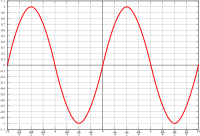
\includegraphics[width=8cm]{mono.png}
			\caption{Onda Monofásica}
			\end{figure}
			La razón del por que se usa este tipo de energía de forma más cotidiana que industrial es tomando de ejemplo los motores monofásicos toman  más energía que los motores trifásicos y por tanto, en este ejemplo encontramos que la energía trifasica es mejor para el tipo de uso industrial
			
			\hspace{3cm}{\huge{\textbf{Trifásica:}}} 
			\\

			\hspace{3.5cm}{Este es el tipo de corriente que consta de 3 fases, tres corrientes alternas distintas que dividen en tres partes las instalaciones a las que llega potencia constante, ésta se encuentra comúnmente en las industrias grandes, que requieren mucho trabajo. Podemos observar este tipo de onda en la \textit{Figura:2}\\}
			\begin{figure}[hbtp]
			\centering
			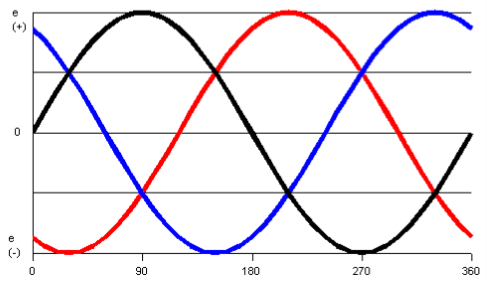
\includegraphics[width=8cm]{Tensiones-trifasicas.png}
			\caption{Onda Trifásica}
			\end{figure}
por tanto podemos observar que es de vital importancia desde el punto de vista de los accionamientos \vspace{.5cm}
dentro de los convertidores monofasicos encontramos:\\ 
\textbf{Los de medio puente[Half bridge]}: y sus caracteristicas son:\\
	\begin{itemize}
	\item	Sus razones topológicas[Razones matemáticas] están perfectamente adecuadas para batería alta y potencia de carga media 
	\item	Tensión máxima en ambos generadores por tanto potencia elevada que en un puente completo 
	\item	Tensión maxima que deben soportar los interruptores de potencia más las sobretensiones que genere los circuitos prácticos 
	\end{itemize}

\textbf{Puente completo[FullBridge]}: Y sus características son:\\
\begin{itemize}
	\item Topología adecuada para tensión alta en una batería 
	\item Puente de n interruptores de potencia 
	\item potencia de corrientes más baja que en el medio puente
	
\end{itemize}
		
\textbf{Puente Pull Push}: ysua características son:\\
	\begin{itemize}
	\item empeora su rendimiento con los circuitos prácticos 
	\item no se aconseja utilizar este tipo de topología para potencias de 10kVA
	\item solo usa dos interruptores de potencia 
	\item habrá inductancia de dispersión del transformador
	\end{itemize}
		}
		 	\vspace{1.5cm}
\begin{center}
\begin{Huge}
\textbf{--Relación de la amplitud de modulación--}
\\
\vspace{1cm}
\end{Huge}
	\begin{huge}
		$m_a = \dfrac{V_{max_{ control}}}{V_{max_{ triangular}}}$
	\end{huge}
\end{center}

\begin{center}
\begin{Huge}
\textbf{--Relación de la frecuencia de modulación--}
\\
\vspace{1cm}
\end{Huge}
	\begin{huge}
		$m_F = \dfrac{F_{triangular}}{V_{onda\_control}}$
	\end{huge}
\end{center}
		 	
\vspace{1cm}

\begin{LARGE}
Entre los controles de tensión de salida por la variación de $m_a$ podemos encontrar los lineales, la sobre modulacion y la onda cuadrada:
\end{LARGE}

\vspace{.5cm}

\begin{Huge}
	 \textbf{Características:}
\end{Huge}

\vspace{.5cm}

\begin{huge}
\hspace{3cm}\textbf{ZonaLineal:}
\end{huge}
\begin{LARGE}
 \begin{itemize}
 	\item La relación que tiene la amplitud de modulación está constituida entre los 0's y 1's
 	\item La amplitud de la componente fundamental es proporcional a $m_a$\\
 
 \end{itemize}
 
\begin{huge}
\hspace{3cm}\textbf{Sobremodulación:}
\end{huge}
\begin{itemize}
	\item Su relación de amplitud es $>$ 1
	\item Crean más armonicos 
\end{itemize}

\end{LARGE}

	
\begin{huge}
\hspace{3cm}\textbf{Onda cuadrada:}
\end{huge}
\begin{LARGE}
\begin{itemize}
	\item La amplitúd de $c_F$ de Ts toma el valor máximo durante todo este periodo
	\item Crean más armonicos 
\end{itemize}
\end{LARGE}

\vspace{1cm}

\begin{flushleft}

















%%CA CA
{\color{cyan}\huge{\textbf{Convertidores: CA-CA:}}}\\
	\vspace{.3cm}
\end{flushleft}
\begin{LARGE}
	Los convertidores CA-CA toman la corriente alterna y la transforman en corriente alterna. pero claro, esto no suena muy útil, pero en realidad si lo es. Toman la corriente alterna y la transforman en otro tipo de corriente alterna con características distintas, como en su valor eficaz[Valor que tendría una corriente continua[CC] que produjera la misma potencia que la corriente alterna de la que se habla], su frecuencia o en los dos.\\
	\vspace{3cm}
	Hay muchos modos de control para reguladores de CA de los cuales los mas utilizados son: 

	\begin{itemize}
	\item control de pasos por cero o por secuencia
	\item por ángulo de fase 
	\item control de amplitúd
	
	\end{itemize}
\end{LARGE}
\vspace{1cm}




















%CC-CC
{\color{cyan}\huge{\textbf{Convertidores: CC-CC:}}}\\
\begin{LARGE}
Este tipo de conversor sirve para convertir los niveles de tensión continua en niveles de tensión continua regulada.\\
Este puede ser de dos tipos: \textbf{Reductor:} que como lo dice su nombre es en el que la tensión de salida es menor que el de entrada y el \textbf{Elevador:} que es aquel que toma la tensión de entrada y la manda mayor como tensión de salida, así logicamente podemos sacar su función.\\	

Dentro de este tipo de conversores econtramos la división de convertidores Boost y los convertidores Buck:\\

	\begin{huge}
	\textbf{Conversor tipo boost}
	\end{huge}\\
	Este tipo de conversor consiste en dos estados, dependiendo claro del interruptor, cuando está abierto y cuando está cerrado como podemos ver en la \textit{figura: 3}.
	 \begin{figure}[hbtp]
	 \centering
	 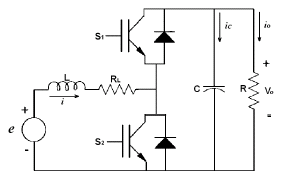
\includegraphics[width=10cm]{boost.png}
	 \caption{Conversor tipo Boost}
	 \end{figure}\\
	\hspace{3cm}\begin{huge}\textbf{$\Rightarrow$[On-State]:}	\end{huge}\\
		Es cuando el interruptor está cerrado, y en este caso la bobina almacena la energía d e la fuente y la carga se hace por un condensador.\\ 
		\vspace{1cm}
	\hspace{3cm}\begin{huge}\textbf{$\Rightarrow$[Off-State]:}	\end{huge}\\
	Es cuando el interruptor está abierto, circula por el diodo y espera hasta que se cargue por completo el condensador para cargarla. \\
	\begin{figure}[hbtp]
	\caption{On/Off state}
	\centering
	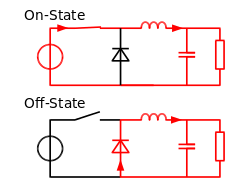
\includegraphics[scale=1]{on-offsstate.png}
	\end{figure}
	
	\vspace{1cm}

	\pagebreak
	\begin{huge}
	\textbf{Conversor tipo Buck}
	\end{huge}\\
	Este convertidor de potencia obtiene una salida menor a la de su entrada y su esquema es bastante parecido al de un conversor tipo Boost es decir una fuente conmutada con dos dispositivos semiconductores[los transistores y diodos] un inductor y posiblemente un condensador en la salida.\\
	Éste conversor es usado para reducir tensión en circuitos y tiene una gran eficiencia con circuitos integrados y de autoregulación, este tiene dos modos; el continuo y el discontinuo.\\
	\vspace{1.3cm}
	
	
	
	\hspace{3cm}\begin{huge} \textbf{Modo continuo}	\end{huge}\\
	Se puede decir que está en este modo si la corriente que pasa por el inductor[la bobina]no baja a cero durante el ciclo de conmutación	\\
	\vspace{1cm}
	\hspace{3cm}\begin{huge} \textbf{Modo discontinuo}	\end{huge}\\
	La unica diferencia que hay es que el inductor [la bobina] está completamente descargada cuando termina el ciclo de conmutación.\\
	
	
\end{LARGE}

\vspace{2cm}









{\color{cyan}\huge{\textbf{Convertidores: CC-CA:}}}\\
\begin{LARGE}
Este tipo de convertidor toma la corriente continua y la transforma en corriente alterna, con la utilización de distintos metodos como:\\
	\hspace{3cm}\begin{huge}\textbf{Convertidor trifásico: }\end{huge}\\
	Estos son utilizados para alimentación de cargas trifásicas que requieran de la corriente alterna y se caracterizan por sus aplicaciones que son las fuentes de voltaje alterno trifásicas pero sin interrupciones, conexión de fuentes que producen energía continua con las cargas trifásicas. Este circuito lo podemos ver en la \textit{figura: 5}\\
	\begin{figure}[hbtp]
	\centering
	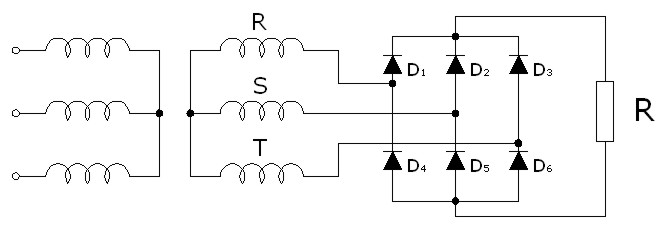
\includegraphics[scale=1]{trifasico.jpg}
	\caption{Convertidor Trifásico}
	\end{figure}
	\vspace{3cm}
\hspace{3cm}\begin{huge}\textbf{Modo Deltha: }\end{huge}\\
	En delta encontramos que los inductores están unidos en un triángulo tal como en la letra griega Delta [$\Delta$] como podemos observar en la \textit{figura:6}
	\begin{figure}[hbtp]
	\centering
	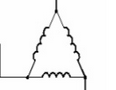
\includegraphics[width=10cm]{delta.png}
	\caption{Delta $\Delta$}
	\end{figure}
	
También los podemos incluir en forma de estrella con el tipo de circuito del mismo nombre como lo podemos ver en la \textit{Figura: 7}\\
\begin{figure}[hbtp]
\centering
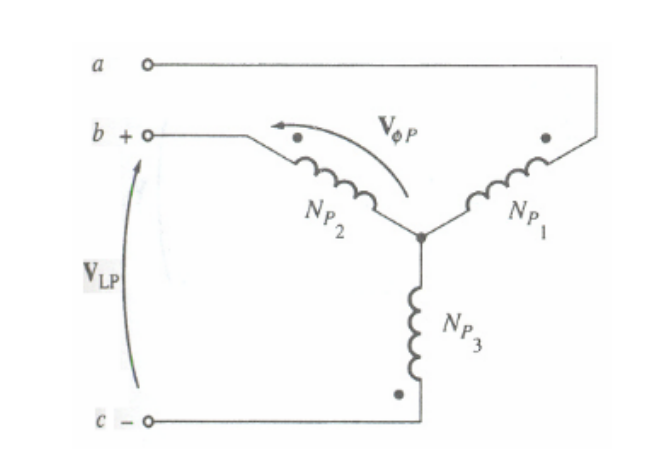
\includegraphics[width=10cm]{star.png}
\caption{Star mode}
\end{figure}
\vspace{1cm}

Y estos son para convertir de corriente continua[CC] a corriente alterna[CA].
\pagebreak

\hspace{3cm}\begin{huge}\textbf{Convertidor Monofásico: }\end{huge}\\


Este tipo de convertidor toma lo que es la corriente continua y la transforma en corriente alterna, generando una pequeña perdida en la conmutación de la energía en energía alterna, para poder entender sus caracteristicas y el como lo hace debemos saber que es su \textbf{topología}, que es un \textbf{inversor de medio puente} y como controlar este inversor.\\
\vspace{.7cm}
\begin{Huge}
	\hspace{3cm} \textbf{Topología: }\\
		\vspace{.3cm}
		
\end{Huge} 
Como topología encontramos que se basa en la conexión de relevadores monofásicos en serie, con fuentes de alimentación impedantes y cada uno de los inversores monofásicos genera tres salidas de tensión de corriente alterna.\\ 
\vspace{.7cm}
\begin{Huge}
	\hspace{3cm} \textbf{Inversor de medio puente: }\\
		\vspace{.3cm}
\end{Huge} 		
Tomamos los capacitores 1 y 2 é imaginemos que están cargados a la mitad del voltaje  $V_s$ cuando pasa por todo el proceso podemos obtener una onda de señal cuadrada y para la segunda parte de su periodo obtendremos la misma onda pero de manera inversa como podemos ver en la \textit{figura: 8}.\\
\vspace{.8cm}
\begin{figure}[hbtp]
\centering
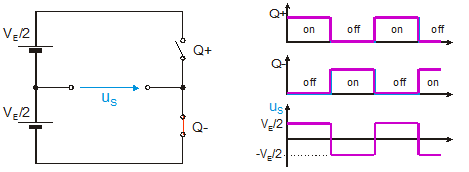
\includegraphics[scale=1]{Inversormediopuente.png}
\caption{Inversor de medio puente monofásico}
\end{figure}

Y para poder entender este inversor debemos analizar el control de un inversor de meido puente.\\

\begin{Huge}
	\hspace{3cm} \textbf{Control inversor de medio puente: }\\
		\vspace{.3cm}
\end{Huge} 
Se encuentra en una tabla de inversores de medio puente en donde vemos que pasa si todos los interruptores están cerrados, si 'A' está cerrado y 'B' abierto y viseversa. 


\end{LARGE}		 				 		
		 	

\end{flushleft}

}
\end{document}
